% ft-05-ExponentialFunctions.tex

\documentclass[xcolor=dvipsnames]{beamer}

\usepackage{cancel}
\renewcommand{\CancelColor}{\color{red}}
\usepackage{graphicx}
\usepackage{wrapfig}
\usepackage{colortbl}
\usepackage{color}
\usepackage{alltt}
\renewcommand*{\thefootnote}{\fnsymbol{footnote}}
\definecolor{myblue}{rgb}{0.8,0.85,1}

\mode<presentation>
{
  \usetheme{Warsaw}
  \setbeamercovered{transparent}
}
% \usecolortheme[named=OliveGreen]{structure}
\setbeamertemplate{navigation symbols}{} 
\setbeamertemplate{blocks}[rounded][shadow=true] 

% this is for overlaying math symbols, see https://tex.stackexchange.com/questions/12895/overlay-symbol-with-another
\def\qeq{\mathrel{%
    \mathchoice{\QEQ}{\QEQ}{\scriptsize\QEQ}{\tiny\QEQ}%
}}
\def\QEQ{{%
    \setbox0\hbox{$\longrightarrow$}%
    \rlap{\hbox to \wd0{\hss/\hss}}\box0
  }}

\newcounter{expls}
\setcounter{expls}{0}
\newcommand{\beispiel}[1]{\refstepcounter{expls}\textbf{Example \arabic{expls}: #1.}}

\newcounter{exercise}
\setcounter{exercise}{0}
\newcommand{\ubung}[0]{\refstepcounter{exercise}\textbf{Exercise \arabic{exercise}: }}

\newif\ifBCITCourse
\BCITCoursetrue
% \BCITCoursefalse
\newif\ifWhichCourse
\WhichCoursetrue
% \WhichCoursefalse
\ifBCITCourse
\ifWhichCourse
\newcommand{\CourseName}{Technical Mathematics for Food Technology}
\newcommand{\CourseNumber}{MATH 1441}
\newcommand{\CourseInst}{BCIT}
\else
\newcommand{\CourseName}{Technical Mathematics for Geomatics}
\newcommand{\CourseNumber}{MATH 1511}
\newcommand{\CourseInst}{BCIT}
\fi
\else
\newcommand{\CourseName}{Philosophy and Literature}
\newcommand{\CourseNumber}{PHIL 375}
\newcommand{\CourseInst}{UBC}
\fi

\title{Exponential Functions}
\subtitle{{\CourseNumber}, BCIT}

\author{\CourseName}

\date{September 21, 2017}

\begin{document}

\begin{frame}
  \titlepage
\end{frame}

\begin{frame}
  \frametitle{Natural Exponents}
(This has been improved in gm-10-exponents.tex.)

Here is how exponents are defined for positive integers,
\begin{equation}
  \label{eq:ogheenoo}
  \begin{array}{rcl}
    a^{n}&=&\underbrace{a\cdot\ldots\cdot{}a} \\
         &&n\mbox{ times}
  \end{array}
\end{equation}
$a$ is called the \alert{base}, $n$ is called the \alert{exponent}.
But how will we define an exponential expression if the base is
negative, a fraction, or irrational?
\end{frame}

\begin{frame}
  \frametitle{Integer Exponents}
Notice that
\begin{equation}
  \label{eq:xeimuoch}
  \frac{a^{n}}{a^{m}}=a^{n-m}
\end{equation}
if $n>m$. If we want (\ref{eq:xeimuoch}) to be true when $n=m$ or
$n<m$, then integer exponents must be defined as follows,
\begin{equation}
  \label{eq:raishaep}
  a^{0}=1
\end{equation}
\begin{equation}
  \label{eq:pahcahka}
  a^{-n}=\frac{1}{a^{n}}\mbox{ for a positive integer }n
\end{equation}
\end{frame}

\begin{frame}
  \frametitle{Integer Exponents Pattern}
  \begin{figure}[h]
    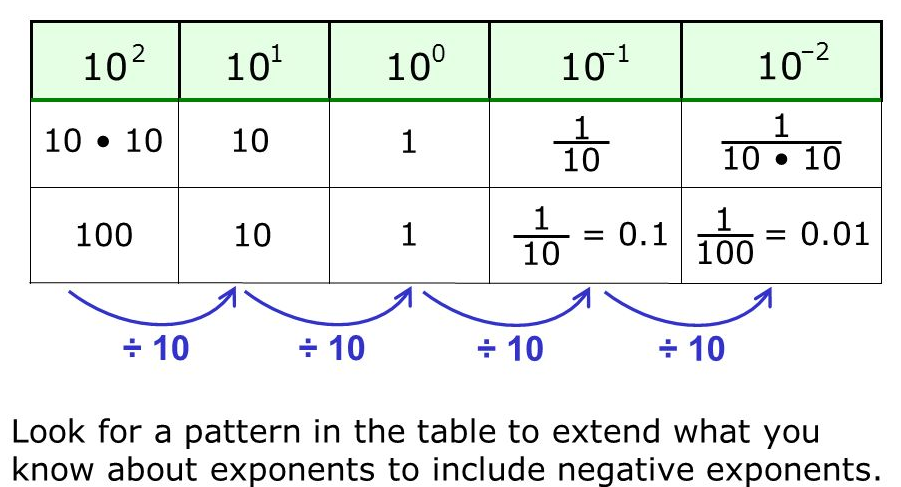
\includegraphics[scale=.4]{./IntegerExponentsPattern.png}
  \end{figure}
\end{frame}

\begin{frame}
  \frametitle{Rational Exponents}
Notice that
\begin{equation}
  \label{eq:ohxukiab}
  \left(a^{n}\right)^{m}=a^{n\cdot{}m}
\end{equation}
for positive integers $n$ and $m$. If we want (\ref{eq:ohxukiab}) to
be true for exponents of the form $\frac{1}{n}$ for an integer $n$,
then the following must be true of them,
\begin{equation}
  \label{eq:aivienai}
  \left(a^{\frac{1}{n}}\right)^{n}=a^{\frac{1}{n}\cdot{}n}=a
\end{equation}
and therefore
\begin{equation}
  \label{eq:kaohahae}
  a^{\frac{1}{n}}=\sqrt[n]{a}
\end{equation}
\end{frame}

\begin{frame}
  \frametitle{Rational and Real Exponents}
In order to get
\begin{equation}
  \label{eq:yahdahse}
  a^{\frac{1}{n}}=\sqrt[n]{a}
\end{equation}
let us define expressions with a fraction as exponent as follows,
\begin{equation}
  \label{eq:aiweelef}
  a^{\frac{m}{n}}=\sqrt[n]{a^{m}}
\end{equation}
Irrational numbers are the limit of a sequence of rational numbers, so
for any real number $c$ there is a sequence such that
$\lim_{k\rightarrow{}\infty}c_{k}=c$, where all $c_{k}$ are rational.
Let us define expressions with an irrational number $c$ as exponent as
follows,
\begin{equation}
  \label{eq:iefiemae}
  a^{c}=\lim_{k\rightarrow{}\infty}a^{c_{k}}
\end{equation}
\end{frame}

\begin{frame}
  \frametitle{Laws of Exponents}
Now we have the following laws,
\begin{equation}
  \label{eq:eihietae}
  a^{x}\cdot{}a^{y}=a^{x+y}
\end{equation}
\begin{equation}
  \label{eq:eeyaidie}
  \frac{a^{x}}{a^{y}}=a^{x-y}
\end{equation}
\begin{equation}
  \label{eq:ieboonge}
  \left(a^{x}\right)^{y}=a^{x\cdot{}y}
\end{equation}
\begin{equation}
  \label{eq:oongenoh}
  (ab)^{x}=a^{x}b^{x}
\end{equation}
\begin{equation}
  \label{eq:rahsieti}
  \left(\frac{a}{b}\right)^{x}=\frac{a^{x}}{b^{x}}
\end{equation}
\end{frame}

\begin{frame}
  \frametitle{Radicals}
  Note that the laws of exponents also apply to expressions under a
  root sign, sometimes called \alert{radicals}, because
  \begin{equation}
    \label{eq:shoaphoo}
    \sqrt{a}=a^{\frac{1}{2}}
  \end{equation}
  \begin{equation}
    \label{eq:thishoof}
    \sqrt[m]{a}=a^{\frac{1}{m}}
  \end{equation}
  Therefore,
  \begin{equation}
    \label{eq:oisheidu}
    \sqrt[m]{a\cdot{}b}=\sqrt[m]{a}\cdot\sqrt[m]{b}
  \end{equation}
  \begin{equation}
    \label{eq:xahpiesh}
    \sqrt[m]{\frac{a}{b}}=\frac{\sqrt[m]{a}}{\sqrt[m]{b}}
  \end{equation}
  but
  \begin{equation}
    \label{eq:ucaithoh}
    \sqrt[m]{a+b}\alert{\neq}\sqrt[m]{a}+\sqrt[m]{b}
  \end{equation}
  \begin{equation}
    \label{eq:quohseiy}
    \sqrt[m]{a-b}\alert{\neq}\sqrt[m]{a}-\sqrt[m]{b}
  \end{equation}
\end{frame}

\begin{frame}
  \frametitle{Exercises}
Simplify the following expressions,
\begin{equation}
  \label{eq:ohahgaoy}
  16^{\frac{7}{4}}\cdot{}16^{-\frac{1}{2}}
\end{equation}
\begin{equation}
  \label{eq:ungeipau}
  \frac{8^{\frac{5}{3}}}{8^{-\frac{1}{3}}}
\end{equation}
\begin{equation}
  \label{eq:zaiquahu}
  \left(64^{\frac{4}{3}}\right)^{-\frac{1}{2}}
\end{equation}
\begin{equation}
  \label{eq:uobeigha}
  (16\cdot{}81)^{-\frac{1}{4}}
\end{equation}
\begin{equation}
  \label{eq:neeshaej}
  \left(\frac{3^{\frac{1}{2}}}{2^{\frac{1}{3}}}\right)^{4}
\end{equation}
\end{frame}

\begin{frame}
  \frametitle{Exercises}
Simplify the following expressions,
\begin{equation}
  \label{eq:phiuchai}
\left[\left(-\frac{5ax^{2}}{3b^{2}y}\right)^{4}\div\left(\frac{5ax}{12b^{3}y^{2}}\right)^{3}\right]\cdot\left(\frac{by}{2ax}\right)^{4}
\end{equation}
\begin{equation}
  \label{eq:taejahbo}
\sqrt[3]{108}-\sqrt[3]{32}
\end{equation}
\begin{equation}
  \label{eq:aineivee}
(2s^{3}t^{-1})\left(\frac{1}{4}s^{6}\right)(16t^{4})
\end{equation}
\begin{equation}
  \label{eq:woongais}
(3ab^{2}c)\left(\frac{2a^{2}b}{c^{3}}\right)^{-2}
\end{equation}
\begin{equation}
  \label{eq:waitaeku}
\frac{2v+3w}{\sqrt{4v^{2}-9w^{2}}}
\end{equation}
\end{frame}

\begin{frame}
  \frametitle{The Exponential Function: Graph}
Let's have a look at the graph for the exponential function.
  \begin{figure}[h]
    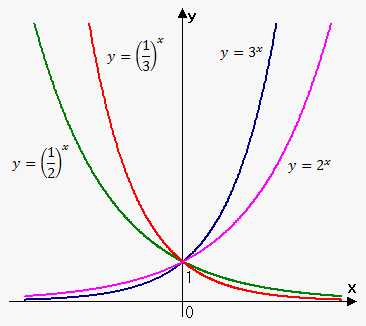
\includegraphics[scale=.6]{./1_2_exponential_function.png}
  \end{figure}
\end{frame}

\begin{frame}
  \frametitle{The Exponential Function: Properties}
  Here are some properties for the following exponential function
  ($a>0$),
\begin{equation}
  \label{eq:muwauzie}
  f(x)=a^{x}
\end{equation}
\end{frame}

\begin{frame}
  \frametitle{The Exponential Function: Properties}
\begin{itemize}
\item<1-> if $a=1$ then the exponential function is the constant function $f(x)=1$
\item<2-> $f(0)=1$ and $f(1)=a$
\item<3-> the domain of $f$ is the real numbers, the range of $f$ is
  all positive real numbers, and $f$ is injective (one-to-one)
\item<4-> if $a>1$ then $f(x)$ tends to $0$ as $x\rightarrow -\infty$, and
  $f(x)$ goes very fast to $+\infty$ as $x\rightarrow \infty$
\item<5-> if $a<1$ then $f(x)$ tends to $0$ as $x\rightarrow \infty$, and
  $f(x)$ goes very fast to $+\infty$ as $x\rightarrow -\infty$
\item<6-> how fast the graph rises to $+\infty$ on the left or the
  right depends on how large $a$ is (if $a>1$) or how small
  $a$ is (if $a<1$). The closer $a$ is to $1$, the flatter the graph.
  `Flat,' of course, is a relative term here: no matter how close $a$
  is to $1$, the function graph will still rise faster than any polynomial.
\end{itemize}
\end{frame}

\begin{frame}
  \frametitle{Euler's Number}
It is convenient to agree on a base that we will use most of the time
(just as 10 is the base for our decimal system, even though it could
be any other natural number greater than 1). 2 or 10 are obvious
candidates, but it turns out that another number, which is irrational,
has special properties in calculus. We call this number $e$ (Euler's
number). It is the limit of the following series (infinite addition),
\begin{equation}
  \label{eq:ohxairei}
    e=\frac{1}{1}+\frac{1}{1}+\frac{1}{1\cdot 2}+\frac{1}{1\cdot 2\cdot
    3}+\frac{1}{1\cdot 2\cdot 3\cdot 4}+\ldots
\end{equation}
It is also the limit of a sequence (infinite sequence of numbers),
\begin{equation}
  \label{eq:eyalachi}
  e=\lim_{m\rightarrow\infty}\left(1+\frac{1}{m}\right)^{m}
\end{equation}
\end{frame}

\begin{frame}
  \frametitle{Exercises}
  {\ubung} Simplify the following expression,
\begin{equation}
  \label{eq:eedeezoh}
  \left(\frac{x^{3}}{-27y^{-6}}\right)^{-\frac{2}{3}}
\end{equation}
\end{frame}

\begin{frame}
  \frametitle{Exercises}
  {\ubung} Simplify the following expression,
\begin{equation}
  \label{eq:eajaekei}
  \left(\frac{x^{-3}}{y^{-2}}\right)^{2}\left(\frac{y}{x}\right)^{4}
\end{equation}
\end{frame}

\begin{frame}
  \frametitle{Exercises}
  {\ubung} Simplify the following expression,
\begin{equation}
  \label{eq:ohchoewi}
  \sqrt[3]{x^{-2}}\cdot\sqrt{4x^{5}}
\end{equation}
\end{frame}

\begin{frame}
  \frametitle{Exercises}
  {\ubung} Evaluate the following expression,
\begin{equation}
  \label{eq:ohzeiphi}
  \left(\frac{7^{-5}\cdot{}7^{2}}{7^{-2}}\right)^{-1}
\end{equation}
\end{frame}

\begin{frame}
  \frametitle{Exercises}
  {\ubung} Evaluate the following expression,
\begin{equation}
  \label{eq:puareipo}
  \sqrt[3]{\frac{-8}{27}}
\end{equation}
\end{frame}

\begin{frame}
  \frametitle{Exercises}
  {\ubung} Evaluate the following expression,
\begin{equation}
  \label{eq:eteequod}
  \left(\frac{1}{\sqrt{3}}\right)^{0}
\end{equation}
\end{frame}

\begin{frame}
  \frametitle{End of Lesson}
Next Lesson: Logarithmic Functions.
\end{frame}

\end{document}

